% !TEX encoding = UTF-8 Unicode
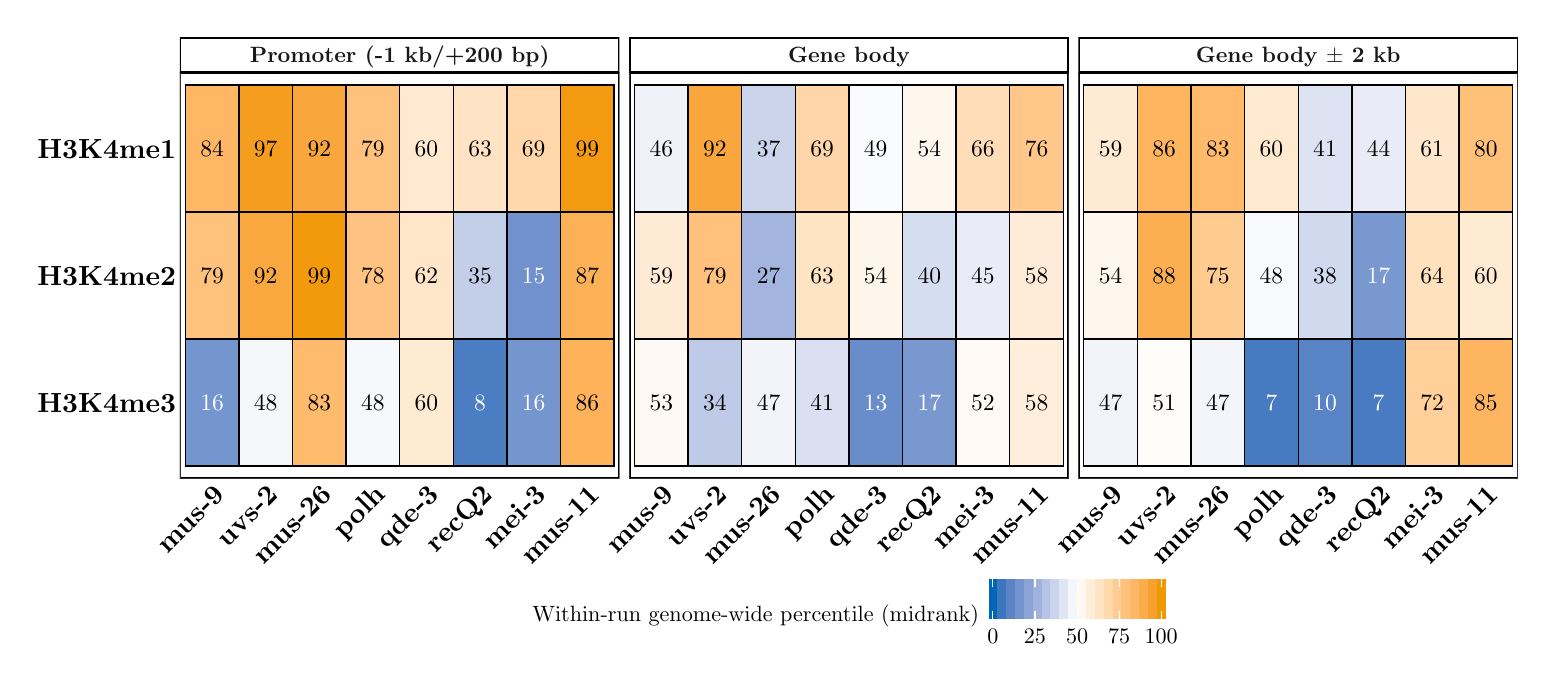
\begin{tikzpicture}[x=1pt,y=1pt]
\definecolor{fillColor}{RGB}{255,255,255}
\path[use as bounding box,fill=fillColor,fill opacity=0.00] (0,0) rectangle (542.02,231.26);
\begin{scope}
\path[clip] (  0.00,  0.00) rectangle (542.02,231.26);
\definecolor{drawColor}{RGB}{255,255,255}
\definecolor{fillColor}{RGB}{255,255,255}

\path[draw=drawColor,line width= 0.7pt,line join=round,line cap=round,fill=fillColor] ( -0.00,  0.00) rectangle (542.02,231.26);
\end{scope}
\begin{scope}
\path[clip] ( 55.01, 68.29) rectangle (213.85,215.09);
\definecolor{drawColor}{RGB}{0,0,0}
\definecolor{fillColor}{RGB}{255,255,255}

\path[draw=drawColor,line width= 1.1pt,line join=round,line cap=round,fill=fillColor] ( 55.01, 68.29) rectangle (213.85,215.09);
\definecolor{fillColor}{RGB}{255,183,101}

\path[draw=drawColor,line width= 0.5pt,fill=fillColor] ( 56.94,164.62) rectangle ( 76.31,210.50);
\definecolor{fillColor}{RGB}{245,157,30}

\path[draw=drawColor,line width= 0.5pt,fill=fillColor] ( 76.31,164.62) rectangle ( 95.68,210.50);
\definecolor{fillColor}{RGB}{249,167,61}

\path[draw=drawColor,line width= 0.5pt,fill=fillColor] ( 95.68,164.62) rectangle (115.05,210.50);
\definecolor{fillColor}{RGB}{255,194,125}

\path[draw=drawColor,line width= 0.5pt,fill=fillColor] (115.05,164.62) rectangle (134.43,210.50);
\definecolor{fillColor}{RGB}{255,233,209}

\path[draw=drawColor,line width= 0.5pt,fill=fillColor] (134.43,164.62) rectangle (153.80,210.50);
\definecolor{fillColor}{RGB}{255,227,196}

\path[draw=drawColor,line width= 0.5pt,fill=fillColor] (153.80,164.62) rectangle (173.17,210.50);
\definecolor{fillColor}{RGB}{255,215,170}

\path[draw=drawColor,line width= 0.5pt,fill=fillColor] (173.17,164.62) rectangle (192.54,210.50);
\definecolor{fillColor}{RGB}{243,154,17}

\path[draw=drawColor,line width= 0.5pt,fill=fillColor] (192.54,164.62) rectangle (211.91,210.50);
\definecolor{fillColor}{RGB}{255,194,124}

\path[draw=drawColor,line width= 0.5pt,fill=fillColor] ( 56.94,118.75) rectangle ( 76.31,164.62);
\definecolor{fillColor}{RGB}{249,168,64}

\path[draw=drawColor,line width= 0.5pt,fill=fillColor] ( 76.31,118.75) rectangle ( 95.68,164.62);
\definecolor{fillColor}{RGB}{243,154,12}

\path[draw=drawColor,line width= 0.5pt,fill=fillColor] ( 95.68,118.75) rectangle (115.05,164.62);
\definecolor{fillColor}{RGB}{255,195,129}

\path[draw=drawColor,line width= 0.5pt,fill=fillColor] (115.05,118.75) rectangle (134.43,164.62);
\definecolor{fillColor}{RGB}{255,230,201}

\path[draw=drawColor,line width= 0.5pt,fill=fillColor] (134.43,118.75) rectangle (153.80,164.62);
\definecolor{fillColor}{RGB}{195,206,233}

\path[draw=drawColor,line width= 0.5pt,fill=fillColor] (153.80,118.75) rectangle (173.17,164.62);
\definecolor{fillColor}{RGB}{113,146,205}

\path[draw=drawColor,line width= 0.5pt,fill=fillColor] (173.17,118.75) rectangle (192.54,164.62);
\definecolor{fillColor}{RGB}{253,177,87}

\path[draw=drawColor,line width= 0.5pt,fill=fillColor] (192.54,118.75) rectangle (211.91,164.62);
\definecolor{fillColor}{RGB}{116,149,206}

\path[draw=drawColor,line width= 0.5pt,fill=fillColor] ( 56.94, 72.87) rectangle ( 76.31,118.75);
\definecolor{fillColor}{RGB}{246,247,251}

\path[draw=drawColor,line width= 0.5pt,fill=fillColor] ( 76.31, 72.87) rectangle ( 95.68,118.75);
\definecolor{fillColor}{RGB}{255,187,108}

\path[draw=drawColor,line width= 0.5pt,fill=fillColor] ( 95.68, 72.87) rectangle (115.05,118.75);
\definecolor{fillColor}{RGB}{247,248,251}

\path[draw=drawColor,line width= 0.5pt,fill=fillColor] (115.05, 72.87) rectangle (134.43,118.75);
\definecolor{fillColor}{RGB}{255,234,210}

\path[draw=drawColor,line width= 0.5pt,fill=fillColor] (134.43, 72.87) rectangle (153.80,118.75);
\definecolor{fillColor}{RGB}{75,125,194}

\path[draw=drawColor,line width= 0.5pt,fill=fillColor] (153.80, 72.87) rectangle (173.17,118.75);
\definecolor{fillColor}{RGB}{117,149,206}

\path[draw=drawColor,line width= 0.5pt,fill=fillColor] (173.17, 72.87) rectangle (192.54,118.75);
\definecolor{fillColor}{RGB}{254,179,91}

\path[draw=drawColor,line width= 0.5pt,fill=fillColor] (192.54, 72.87) rectangle (211.91,118.75);

\node[text=drawColor,anchor=base,inner sep=0pt, outer sep=0pt, scale=  0.85] at ( 66.63,184.62) {84};

\node[text=drawColor,anchor=base,inner sep=0pt, outer sep=0pt, scale=  0.85] at ( 86.00,184.62) {97};

\node[text=drawColor,anchor=base,inner sep=0pt, outer sep=0pt, scale=  0.85] at (105.37,184.62) {92};

\node[text=drawColor,anchor=base,inner sep=0pt, outer sep=0pt, scale=  0.85] at (124.74,184.62) {79};

\node[text=drawColor,anchor=base,inner sep=0pt, outer sep=0pt, scale=  0.85] at (144.11,184.62) {60};

\node[text=drawColor,anchor=base,inner sep=0pt, outer sep=0pt, scale=  0.85] at (163.48,184.62) {63};

\node[text=drawColor,anchor=base,inner sep=0pt, outer sep=0pt, scale=  0.85] at (182.85,184.62) {69};

\node[text=drawColor,anchor=base,inner sep=0pt, outer sep=0pt, scale=  0.85] at (202.22,184.62) {99};

\node[text=drawColor,anchor=base,inner sep=0pt, outer sep=0pt, scale=  0.85] at ( 66.63,138.75) {79};

\node[text=drawColor,anchor=base,inner sep=0pt, outer sep=0pt, scale=  0.85] at ( 86.00,138.75) {92};

\node[text=drawColor,anchor=base,inner sep=0pt, outer sep=0pt, scale=  0.85] at (105.37,138.75) {99};

\node[text=drawColor,anchor=base,inner sep=0pt, outer sep=0pt, scale=  0.85] at (124.74,138.75) {78};

\node[text=drawColor,anchor=base,inner sep=0pt, outer sep=0pt, scale=  0.85] at (144.11,138.75) {62};

\node[text=drawColor,anchor=base,inner sep=0pt, outer sep=0pt, scale=  0.85] at (163.48,138.75) {35};
\definecolor{drawColor}{RGB}{255,255,255}

\node[text=drawColor,anchor=base,inner sep=0pt, outer sep=0pt, scale=  0.85] at (182.85,138.75) {15};
\definecolor{drawColor}{RGB}{0,0,0}

\node[text=drawColor,anchor=base,inner sep=0pt, outer sep=0pt, scale=  0.85] at (202.22,138.75) {87};
\definecolor{drawColor}{RGB}{255,255,255}

\node[text=drawColor,anchor=base,inner sep=0pt, outer sep=0pt, scale=  0.85] at ( 66.63, 92.87) {16};
\definecolor{drawColor}{RGB}{0,0,0}

\node[text=drawColor,anchor=base,inner sep=0pt, outer sep=0pt, scale=  0.85] at ( 86.00, 92.87) {48};

\node[text=drawColor,anchor=base,inner sep=0pt, outer sep=0pt, scale=  0.85] at (105.37, 92.87) {83};

\node[text=drawColor,anchor=base,inner sep=0pt, outer sep=0pt, scale=  0.85] at (124.74, 92.87) {48};

\node[text=drawColor,anchor=base,inner sep=0pt, outer sep=0pt, scale=  0.85] at (144.11, 92.87) {60};
\definecolor{drawColor}{RGB}{255,255,255}

\node[text=drawColor,anchor=base,inner sep=0pt, outer sep=0pt, scale=  0.85] at (163.48, 92.87) {8};

\node[text=drawColor,anchor=base,inner sep=0pt, outer sep=0pt, scale=  0.85] at (182.85, 92.87) {16};
\definecolor{drawColor}{RGB}{0,0,0}

\node[text=drawColor,anchor=base,inner sep=0pt, outer sep=0pt, scale=  0.85] at (202.22, 92.87) {86};
\definecolor{drawColor}{gray}{0.20}

\path[draw=drawColor,line width= 0.7pt,line join=round,line cap=round] ( 55.01, 68.29) rectangle (213.85,215.09);
\end{scope}
\begin{scope}
\path[clip] (217.35, 68.29) rectangle (376.19,215.09);
\definecolor{drawColor}{RGB}{0,0,0}
\definecolor{fillColor}{RGB}{255,255,255}

\path[draw=drawColor,line width= 1.1pt,line join=round,line cap=round,fill=fillColor] (217.35, 68.29) rectangle (376.19,215.09);
\definecolor{fillColor}{RGB}{239,242,249}

\path[draw=drawColor,line width= 0.5pt,fill=fillColor] (219.28,164.62) rectangle (238.65,210.50);
\definecolor{fillColor}{RGB}{249,167,60}

\path[draw=drawColor,line width= 0.5pt,fill=fillColor] (238.65,164.62) rectangle (258.02,210.50);
\definecolor{fillColor}{RGB}{202,213,236}

\path[draw=drawColor,line width= 0.5pt,fill=fillColor] (258.02,164.62) rectangle (277.39,210.50);
\definecolor{fillColor}{RGB}{255,214,169}

\path[draw=drawColor,line width= 0.5pt,fill=fillColor] (277.39,164.62) rectangle (296.77,210.50);
\definecolor{fillColor}{RGB}{250,251,253}

\path[draw=drawColor,line width= 0.5pt,fill=fillColor] (296.77,164.62) rectangle (316.14,210.50);
\definecolor{fillColor}{RGB}{255,247,237}

\path[draw=drawColor,line width= 0.5pt,fill=fillColor] (316.14,164.62) rectangle (335.51,210.50);
\definecolor{fillColor}{RGB}{255,221,185}

\path[draw=drawColor,line width= 0.5pt,fill=fillColor] (335.51,164.62) rectangle (354.88,210.50);
\definecolor{fillColor}{RGB}{255,199,138}

\path[draw=drawColor,line width= 0.5pt,fill=fillColor] (354.88,164.62) rectangle (374.25,210.50);
\definecolor{fillColor}{RGB}{255,235,213}

\path[draw=drawColor,line width= 0.5pt,fill=fillColor] (219.28,118.75) rectangle (238.65,164.62);
\definecolor{fillColor}{RGB}{255,193,123}

\path[draw=drawColor,line width= 0.5pt,fill=fillColor] (238.65,118.75) rectangle (258.02,164.62);
\definecolor{fillColor}{RGB}{163,181,222}

\path[draw=drawColor,line width= 0.5pt,fill=fillColor] (258.02,118.75) rectangle (277.39,164.62);
\definecolor{fillColor}{RGB}{255,228,196}

\path[draw=drawColor,line width= 0.5pt,fill=fillColor] (277.39,118.75) rectangle (296.77,164.62);
\definecolor{fillColor}{RGB}{255,246,235}

\path[draw=drawColor,line width= 0.5pt,fill=fillColor] (296.77,118.75) rectangle (316.14,164.62);
\definecolor{fillColor}{RGB}{213,221,240}

\path[draw=drawColor,line width= 0.5pt,fill=fillColor] (316.14,118.75) rectangle (335.51,164.62);
\definecolor{fillColor}{RGB}{233,236,247}

\path[draw=drawColor,line width= 0.5pt,fill=fillColor] (335.51,118.75) rectangle (354.88,164.62);
\definecolor{fillColor}{RGB}{255,236,216}

\path[draw=drawColor,line width= 0.5pt,fill=fillColor] (354.88,118.75) rectangle (374.25,164.62);
\definecolor{fillColor}{RGB}{255,249,243}

\path[draw=drawColor,line width= 0.5pt,fill=fillColor] (219.28, 72.87) rectangle (238.65,118.75);
\definecolor{fillColor}{RGB}{190,202,231}

\path[draw=drawColor,line width= 0.5pt,fill=fillColor] (238.65, 72.87) rectangle (258.02,118.75);
\definecolor{fillColor}{RGB}{243,244,250}

\path[draw=drawColor,line width= 0.5pt,fill=fillColor] (258.02, 72.87) rectangle (277.39,118.75);
\definecolor{fillColor}{RGB}{218,224,241}

\path[draw=drawColor,line width= 0.5pt,fill=fillColor] (277.39, 72.87) rectangle (296.77,118.75);
\definecolor{fillColor}{RGB}{104,141,202}

\path[draw=drawColor,line width= 0.5pt,fill=fillColor] (296.77, 72.87) rectangle (316.14,118.75);
\definecolor{fillColor}{RGB}{121,152,208}

\path[draw=drawColor,line width= 0.5pt,fill=fillColor] (316.14, 72.87) rectangle (335.51,118.75);
\definecolor{fillColor}{RGB}{255,250,246}

\path[draw=drawColor,line width= 0.5pt,fill=fillColor] (335.51, 72.87) rectangle (354.88,118.75);
\definecolor{fillColor}{RGB}{255,238,219}

\path[draw=drawColor,line width= 0.5pt,fill=fillColor] (354.88, 72.87) rectangle (374.25,118.75);

\node[text=drawColor,anchor=base,inner sep=0pt, outer sep=0pt, scale=  0.85] at (228.97,184.62) {46};

\node[text=drawColor,anchor=base,inner sep=0pt, outer sep=0pt, scale=  0.85] at (248.34,184.62) {92};

\node[text=drawColor,anchor=base,inner sep=0pt, outer sep=0pt, scale=  0.85] at (267.71,184.62) {37};

\node[text=drawColor,anchor=base,inner sep=0pt, outer sep=0pt, scale=  0.85] at (287.08,184.62) {69};

\node[text=drawColor,anchor=base,inner sep=0pt, outer sep=0pt, scale=  0.85] at (306.45,184.62) {49};

\node[text=drawColor,anchor=base,inner sep=0pt, outer sep=0pt, scale=  0.85] at (325.82,184.62) {54};

\node[text=drawColor,anchor=base,inner sep=0pt, outer sep=0pt, scale=  0.85] at (345.19,184.62) {66};

\node[text=drawColor,anchor=base,inner sep=0pt, outer sep=0pt, scale=  0.85] at (364.56,184.62) {76};

\node[text=drawColor,anchor=base,inner sep=0pt, outer sep=0pt, scale=  0.85] at (228.97,138.75) {59};

\node[text=drawColor,anchor=base,inner sep=0pt, outer sep=0pt, scale=  0.85] at (248.34,138.75) {79};

\node[text=drawColor,anchor=base,inner sep=0pt, outer sep=0pt, scale=  0.85] at (267.71,138.75) {27};

\node[text=drawColor,anchor=base,inner sep=0pt, outer sep=0pt, scale=  0.85] at (287.08,138.75) {63};

\node[text=drawColor,anchor=base,inner sep=0pt, outer sep=0pt, scale=  0.85] at (306.45,138.75) {54};

\node[text=drawColor,anchor=base,inner sep=0pt, outer sep=0pt, scale=  0.85] at (325.82,138.75) {40};

\node[text=drawColor,anchor=base,inner sep=0pt, outer sep=0pt, scale=  0.85] at (345.19,138.75) {45};

\node[text=drawColor,anchor=base,inner sep=0pt, outer sep=0pt, scale=  0.85] at (364.56,138.75) {58};

\node[text=drawColor,anchor=base,inner sep=0pt, outer sep=0pt, scale=  0.85] at (228.97, 92.87) {53};

\node[text=drawColor,anchor=base,inner sep=0pt, outer sep=0pt, scale=  0.85] at (248.34, 92.87) {34};

\node[text=drawColor,anchor=base,inner sep=0pt, outer sep=0pt, scale=  0.85] at (267.71, 92.87) {47};

\node[text=drawColor,anchor=base,inner sep=0pt, outer sep=0pt, scale=  0.85] at (287.08, 92.87) {41};
\definecolor{drawColor}{RGB}{255,255,255}

\node[text=drawColor,anchor=base,inner sep=0pt, outer sep=0pt, scale=  0.85] at (306.45, 92.87) {13};

\node[text=drawColor,anchor=base,inner sep=0pt, outer sep=0pt, scale=  0.85] at (325.82, 92.87) {17};
\definecolor{drawColor}{RGB}{0,0,0}

\node[text=drawColor,anchor=base,inner sep=0pt, outer sep=0pt, scale=  0.85] at (345.19, 92.87) {52};

\node[text=drawColor,anchor=base,inner sep=0pt, outer sep=0pt, scale=  0.85] at (364.56, 92.87) {58};
\definecolor{drawColor}{gray}{0.20}

\path[draw=drawColor,line width= 0.7pt,line join=round,line cap=round] (217.35, 68.29) rectangle (376.19,215.09);
\end{scope}
\begin{scope}
\path[clip] (379.69, 68.29) rectangle (538.52,215.09);
\definecolor{drawColor}{RGB}{0,0,0}
\definecolor{fillColor}{RGB}{255,255,255}

\path[draw=drawColor,line width= 1.1pt,line join=round,line cap=round,fill=fillColor] (379.69, 68.29) rectangle (538.53,215.09);
\definecolor{fillColor}{RGB}{255,235,212}

\path[draw=drawColor,line width= 0.5pt,fill=fillColor] (381.62,164.62) rectangle (400.99,210.50);
\definecolor{fillColor}{RGB}{254,181,94}

\path[draw=drawColor,line width= 0.5pt,fill=fillColor] (400.99,164.62) rectangle (420.36,210.50);
\definecolor{fillColor}{RGB}{255,186,107}

\path[draw=drawColor,line width= 0.5pt,fill=fillColor] (420.36,164.62) rectangle (439.73,210.50);
\definecolor{fillColor}{RGB}{255,233,207}

\path[draw=drawColor,line width= 0.5pt,fill=fillColor] (439.73,164.62) rectangle (459.11,210.50);
\definecolor{fillColor}{RGB}{221,227,242}

\path[draw=drawColor,line width= 0.5pt,fill=fillColor] (459.11,164.62) rectangle (478.48,210.50);
\definecolor{fillColor}{RGB}{233,236,247}

\path[draw=drawColor,line width= 0.5pt,fill=fillColor] (478.48,164.62) rectangle (497.85,210.50);
\definecolor{fillColor}{RGB}{255,231,204}

\path[draw=drawColor,line width= 0.5pt,fill=fillColor] (497.85,164.62) rectangle (517.22,210.50);
\definecolor{fillColor}{RGB}{255,192,120}

\path[draw=drawColor,line width= 0.5pt,fill=fillColor] (517.22,164.62) rectangle (536.59,210.50);
\definecolor{fillColor}{RGB}{255,247,237}

\path[draw=drawColor,line width= 0.5pt,fill=fillColor] (381.62,118.75) rectangle (400.99,164.62);
\definecolor{fillColor}{RGB}{252,175,81}

\path[draw=drawColor,line width= 0.5pt,fill=fillColor] (400.99,118.75) rectangle (420.36,164.62);
\definecolor{fillColor}{RGB}{255,203,143}

\path[draw=drawColor,line width= 0.5pt,fill=fillColor] (420.36,118.75) rectangle (439.73,164.62);
\definecolor{fillColor}{RGB}{248,249,252}

\path[draw=drawColor,line width= 0.5pt,fill=fillColor] (439.73,118.75) rectangle (459.11,164.62);
\definecolor{fillColor}{RGB}{208,217,238}

\path[draw=drawColor,line width= 0.5pt,fill=fillColor] (459.11,118.75) rectangle (478.48,164.62);
\definecolor{fillColor}{RGB}{121,152,208}

\path[draw=drawColor,line width= 0.5pt,fill=fillColor] (478.48,118.75) rectangle (497.85,164.62);
\definecolor{fillColor}{RGB}{255,225,190}

\path[draw=drawColor,line width= 0.5pt,fill=fillColor] (497.85,118.75) rectangle (517.22,164.62);
\definecolor{fillColor}{RGB}{255,234,210}

\path[draw=drawColor,line width= 0.5pt,fill=fillColor] (517.22,118.75) rectangle (536.59,164.62);
\definecolor{fillColor}{RGB}{243,244,250}

\path[draw=drawColor,line width= 0.5pt,fill=fillColor] (381.62, 72.87) rectangle (400.99,118.75);
\definecolor{fillColor}{RGB}{255,252,250}

\path[draw=drawColor,line width= 0.5pt,fill=fillColor] (400.99, 72.87) rectangle (420.36,118.75);
\definecolor{fillColor}{RGB}{243,245,251}

\path[draw=drawColor,line width= 0.5pt,fill=fillColor] (420.36, 72.87) rectangle (439.73,118.75);
\definecolor{fillColor}{RGB}{70,123,193}

\path[draw=drawColor,line width= 0.5pt,fill=fillColor] (439.73, 72.87) rectangle (459.11,118.75);
\definecolor{fillColor}{RGB}{88,131,197}

\path[draw=drawColor,line width= 0.5pt,fill=fillColor] (459.11, 72.87) rectangle (478.48,118.75);
\definecolor{fillColor}{RGB}{72,123,193}

\path[draw=drawColor,line width= 0.5pt,fill=fillColor] (478.48, 72.87) rectangle (497.85,118.75);
\definecolor{fillColor}{RGB}{255,208,154}

\path[draw=drawColor,line width= 0.5pt,fill=fillColor] (497.85, 72.87) rectangle (517.22,118.75);
\definecolor{fillColor}{RGB}{254,181,96}

\path[draw=drawColor,line width= 0.5pt,fill=fillColor] (517.22, 72.87) rectangle (536.59,118.75);

\node[text=drawColor,anchor=base,inner sep=0pt, outer sep=0pt, scale=  0.85] at (391.31,184.62) {59};

\node[text=drawColor,anchor=base,inner sep=0pt, outer sep=0pt, scale=  0.85] at (410.68,184.62) {86};

\node[text=drawColor,anchor=base,inner sep=0pt, outer sep=0pt, scale=  0.85] at (430.05,184.62) {83};

\node[text=drawColor,anchor=base,inner sep=0pt, outer sep=0pt, scale=  0.85] at (449.42,184.62) {60};

\node[text=drawColor,anchor=base,inner sep=0pt, outer sep=0pt, scale=  0.85] at (468.79,184.62) {41};

\node[text=drawColor,anchor=base,inner sep=0pt, outer sep=0pt, scale=  0.85] at (488.16,184.62) {44};

\node[text=drawColor,anchor=base,inner sep=0pt, outer sep=0pt, scale=  0.85] at (507.53,184.62) {61};

\node[text=drawColor,anchor=base,inner sep=0pt, outer sep=0pt, scale=  0.85] at (526.90,184.62) {80};

\node[text=drawColor,anchor=base,inner sep=0pt, outer sep=0pt, scale=  0.85] at (391.31,138.75) {54};

\node[text=drawColor,anchor=base,inner sep=0pt, outer sep=0pt, scale=  0.85] at (410.68,138.75) {88};

\node[text=drawColor,anchor=base,inner sep=0pt, outer sep=0pt, scale=  0.85] at (430.05,138.75) {75};

\node[text=drawColor,anchor=base,inner sep=0pt, outer sep=0pt, scale=  0.85] at (449.42,138.75) {48};

\node[text=drawColor,anchor=base,inner sep=0pt, outer sep=0pt, scale=  0.85] at (468.79,138.75) {38};
\definecolor{drawColor}{RGB}{255,255,255}

\node[text=drawColor,anchor=base,inner sep=0pt, outer sep=0pt, scale=  0.85] at (488.16,138.75) {17};
\definecolor{drawColor}{RGB}{0,0,0}

\node[text=drawColor,anchor=base,inner sep=0pt, outer sep=0pt, scale=  0.85] at (507.53,138.75) {64};

\node[text=drawColor,anchor=base,inner sep=0pt, outer sep=0pt, scale=  0.85] at (526.90,138.75) {60};

\node[text=drawColor,anchor=base,inner sep=0pt, outer sep=0pt, scale=  0.85] at (391.31, 92.87) {47};

\node[text=drawColor,anchor=base,inner sep=0pt, outer sep=0pt, scale=  0.85] at (410.68, 92.87) {51};

\node[text=drawColor,anchor=base,inner sep=0pt, outer sep=0pt, scale=  0.85] at (430.05, 92.87) {47};
\definecolor{drawColor}{RGB}{255,255,255}

\node[text=drawColor,anchor=base,inner sep=0pt, outer sep=0pt, scale=  0.85] at (449.42, 92.87) {7};

\node[text=drawColor,anchor=base,inner sep=0pt, outer sep=0pt, scale=  0.85] at (468.79, 92.87) {10};

\node[text=drawColor,anchor=base,inner sep=0pt, outer sep=0pt, scale=  0.85] at (488.16, 92.87) {7};
\definecolor{drawColor}{RGB}{0,0,0}

\node[text=drawColor,anchor=base,inner sep=0pt, outer sep=0pt, scale=  0.85] at (507.53, 92.87) {72};

\node[text=drawColor,anchor=base,inner sep=0pt, outer sep=0pt, scale=  0.85] at (526.90, 92.87) {85};
\definecolor{drawColor}{gray}{0.20}

\path[draw=drawColor,line width= 0.7pt,line join=round,line cap=round] (379.69, 68.29) rectangle (538.53,215.09);
\end{scope}
\begin{scope}
\path[clip] ( 55.01,215.09) rectangle (213.85,227.76);
\definecolor{drawColor}{RGB}{0,0,0}
\definecolor{fillColor}{RGB}{255,255,255}

\path[draw=drawColor,line width= 1.1pt,line join=round,line cap=round,fill=fillColor] ( 55.01,215.09) rectangle (213.85,227.76);
\definecolor{drawColor}{gray}{0.10}

\node[text=drawColor,anchor=base,inner sep=0pt, outer sep=0pt, scale=  0.80] at (134.43,218.67) {\bfseries Promoter (-1 kb/+200 bp)};
\end{scope}
\begin{scope}
\path[clip] (217.35,215.09) rectangle (376.19,227.76);
\definecolor{drawColor}{RGB}{0,0,0}
\definecolor{fillColor}{RGB}{255,255,255}

\path[draw=drawColor,line width= 1.1pt,line join=round,line cap=round,fill=fillColor] (217.35,215.09) rectangle (376.19,227.76);
\definecolor{drawColor}{gray}{0.10}

\node[text=drawColor,anchor=base,inner sep=0pt, outer sep=0pt, scale=  0.80] at (296.77,218.67) {\bfseries Gene body};
\end{scope}
\begin{scope}
\path[clip] (379.69,215.09) rectangle (538.52,227.76);
\definecolor{drawColor}{RGB}{0,0,0}
\definecolor{fillColor}{RGB}{255,255,255}

\path[draw=drawColor,line width= 1.1pt,line join=round,line cap=round,fill=fillColor] (379.69,215.09) rectangle (538.53,227.76);
\definecolor{drawColor}{gray}{0.10}

\node[text=drawColor,anchor=base,inner sep=0pt, outer sep=0pt, scale=  0.80] at (459.11,218.67) {\bfseries Gene body $\pm$ 2 kb};
\end{scope}
\begin{scope}
\path[clip] (  0.00,  0.00) rectangle (542.02,231.26);
\definecolor{drawColor}{RGB}{0,0,0}

\node[text=drawColor,rotate= 45.00,anchor=base east,inner sep=0pt, outer sep=0pt, scale=  1.00] at ( 71.51, 62.01) {\bfseries mus-9};

\node[text=drawColor,rotate= 45.00,anchor=base east,inner sep=0pt, outer sep=0pt, scale=  1.00] at ( 90.88, 62.01) {\bfseries uvs-2};

\node[text=drawColor,rotate= 45.00,anchor=base east,inner sep=0pt, outer sep=0pt, scale=  1.00] at (110.25, 62.01) {\bfseries mus-26};

\node[text=drawColor,rotate= 45.00,anchor=base east,inner sep=0pt, outer sep=0pt, scale=  1.00] at (129.62, 62.01) {\bfseries polh};

\node[text=drawColor,rotate= 45.00,anchor=base east,inner sep=0pt, outer sep=0pt, scale=  1.00] at (148.99, 62.01) {\bfseries qde-3};

\node[text=drawColor,rotate= 45.00,anchor=base east,inner sep=0pt, outer sep=0pt, scale=  1.00] at (168.36, 62.01) {\bfseries recQ2};

\node[text=drawColor,rotate= 45.00,anchor=base east,inner sep=0pt, outer sep=0pt, scale=  1.00] at (187.73, 62.01) {\bfseries mei-3};

\node[text=drawColor,rotate= 45.00,anchor=base east,inner sep=0pt, outer sep=0pt, scale=  1.00] at (207.10, 62.01) {\bfseries mus-11};
\end{scope}
\begin{scope}
\path[clip] (  0.00,  0.00) rectangle (542.02,231.26);
\definecolor{drawColor}{RGB}{0,0,0}

\node[text=drawColor,rotate= 45.00,anchor=base east,inner sep=0pt, outer sep=0pt, scale=  1.00] at (233.85, 62.01) {\bfseries mus-9};

\node[text=drawColor,rotate= 45.00,anchor=base east,inner sep=0pt, outer sep=0pt, scale=  1.00] at (253.22, 62.01) {\bfseries uvs-2};

\node[text=drawColor,rotate= 45.00,anchor=base east,inner sep=0pt, outer sep=0pt, scale=  1.00] at (272.59, 62.01) {\bfseries mus-26};

\node[text=drawColor,rotate= 45.00,anchor=base east,inner sep=0pt, outer sep=0pt, scale=  1.00] at (291.96, 62.01) {\bfseries polh};

\node[text=drawColor,rotate= 45.00,anchor=base east,inner sep=0pt, outer sep=0pt, scale=  1.00] at (311.33, 62.01) {\bfseries qde-3};

\node[text=drawColor,rotate= 45.00,anchor=base east,inner sep=0pt, outer sep=0pt, scale=  1.00] at (330.70, 62.01) {\bfseries recQ2};

\node[text=drawColor,rotate= 45.00,anchor=base east,inner sep=0pt, outer sep=0pt, scale=  1.00] at (350.07, 62.01) {\bfseries mei-3};

\node[text=drawColor,rotate= 45.00,anchor=base east,inner sep=0pt, outer sep=0pt, scale=  1.00] at (369.44, 62.01) {\bfseries mus-11};
\end{scope}
\begin{scope}
\path[clip] (  0.00,  0.00) rectangle (542.02,231.26);
\definecolor{drawColor}{RGB}{0,0,0}

\node[text=drawColor,rotate= 45.00,anchor=base east,inner sep=0pt, outer sep=0pt, scale=  1.00] at (396.19, 62.01) {\bfseries mus-9};

\node[text=drawColor,rotate= 45.00,anchor=base east,inner sep=0pt, outer sep=0pt, scale=  1.00] at (415.56, 62.01) {\bfseries uvs-2};

\node[text=drawColor,rotate= 45.00,anchor=base east,inner sep=0pt, outer sep=0pt, scale=  1.00] at (434.93, 62.01) {\bfseries mus-26};

\node[text=drawColor,rotate= 45.00,anchor=base east,inner sep=0pt, outer sep=0pt, scale=  1.00] at (454.30, 62.01) {\bfseries polh};

\node[text=drawColor,rotate= 45.00,anchor=base east,inner sep=0pt, outer sep=0pt, scale=  1.00] at (473.67, 62.01) {\bfseries qde-3};

\node[text=drawColor,rotate= 45.00,anchor=base east,inner sep=0pt, outer sep=0pt, scale=  1.00] at (493.04, 62.01) {\bfseries recQ2};

\node[text=drawColor,rotate= 45.00,anchor=base east,inner sep=0pt, outer sep=0pt, scale=  1.00] at (512.41, 62.01) {\bfseries mei-3};

\node[text=drawColor,rotate= 45.00,anchor=base east,inner sep=0pt, outer sep=0pt, scale=  1.00] at (531.78, 62.01) {\bfseries mus-11};
\end{scope}
\begin{scope}
\path[clip] (  0.00,  0.00) rectangle (542.02,231.26);
\definecolor{drawColor}{RGB}{0,0,0}

\node[text=drawColor,anchor=base east,inner sep=0pt, outer sep=0pt, scale=  1.00] at ( 53.61, 92.36) {\bfseries H3K4me3};

\node[text=drawColor,anchor=base east,inner sep=0pt, outer sep=0pt, scale=  1.00] at ( 53.61,138.24) {\bfseries H3K4me2};

\node[text=drawColor,anchor=base east,inner sep=0pt, outer sep=0pt, scale=  1.00] at ( 53.61,184.11) {\bfseries H3K4me1};
\end{scope}
\begin{scope}
\path[clip] (  0.00,  0.00) rectangle (542.02,231.26);
\definecolor{fillColor}{RGB}{255,255,255}

\path[fill=fillColor] (178.83,  3.50) rectangle (414.71, 35.52);
\end{scope}
\begin{scope}
\path[clip] (  0.00,  0.00) rectangle (542.02,231.26);
\definecolor{drawColor}{RGB}{0,0,0}

\node[text=drawColor,anchor=base west,inner sep=0pt, outer sep=0pt, scale=  0.80] at (182.33, 16.75) {Within-run genome-wide percentile (midrank)};
\end{scope}
\begin{scope}
\path[clip] (  0.00,  0.00) rectangle (542.02,231.26);
\definecolor{fillColor}{RGB}{0,103,183}

\path[fill=fillColor] (347.19, 17.56) rectangle (350.39, 32.02);
\definecolor{fillColor}{RGB}{60,118,190}

\path[fill=fillColor] (350.39, 17.56) rectangle (353.59, 32.02);
\definecolor{fillColor}{RGB}{90,132,198}

\path[fill=fillColor] (353.59, 17.56) rectangle (356.79, 32.02);
\definecolor{fillColor}{RGB}{115,148,206}

\path[fill=fillColor] (356.79, 17.56) rectangle (359.99, 32.02);
\definecolor{fillColor}{RGB}{138,164,213}

\path[fill=fillColor] (359.99, 17.56) rectangle (363.19, 32.02);
\definecolor{fillColor}{RGB}{160,179,221}

\path[fill=fillColor] (363.19, 17.56) rectangle (366.39, 32.02);
\definecolor{fillColor}{RGB}{181,196,228}

\path[fill=fillColor] (366.39, 17.56) rectangle (369.59, 32.02);
\definecolor{fillColor}{RGB}{202,212,236}

\path[fill=fillColor] (369.59, 17.56) rectangle (372.79, 32.02);
\definecolor{fillColor}{RGB}{224,229,243}

\path[fill=fillColor] (372.79, 17.56) rectangle (376.00, 32.02);
\definecolor{fillColor}{RGB}{245,246,251}

\path[fill=fillColor] (376.00, 17.56) rectangle (379.20, 32.02);
\definecolor{fillColor}{RGB}{255,249,242}

\path[fill=fillColor] (379.20, 17.56) rectangle (382.40, 32.02);
\definecolor{fillColor}{RGB}{255,237,218}

\path[fill=fillColor] (382.40, 17.56) rectangle (385.60, 32.02);
\definecolor{fillColor}{RGB}{255,227,195}

\path[fill=fillColor] (385.60, 17.56) rectangle (388.80, 32.02);
\definecolor{fillColor}{RGB}{255,216,171}

\path[fill=fillColor] (388.80, 17.56) rectangle (392.00, 32.02);
\definecolor{fillColor}{RGB}{255,205,148}

\path[fill=fillColor] (392.00, 17.56) rectangle (395.20, 32.02);
\definecolor{fillColor}{RGB}{255,194,124}

\path[fill=fillColor] (395.20, 17.56) rectangle (398.40, 32.02);
\definecolor{fillColor}{RGB}{255,183,101}

\path[fill=fillColor] (398.40, 17.56) rectangle (401.60, 32.02);
\definecolor{fillColor}{RGB}{251,173,76}

\path[fill=fillColor] (401.60, 17.56) rectangle (404.80, 32.02);
\definecolor{fillColor}{RGB}{247,162,48}

\path[fill=fillColor] (404.80, 17.56) rectangle (408.00, 32.02);
\definecolor{fillColor}{RGB}{242,152,0}

\path[fill=fillColor] (408.00, 17.56) rectangle (411.21, 32.02);
\end{scope}
\begin{scope}
\path[clip] (  0.00,  0.00) rectangle (542.02,231.26);
\definecolor{drawColor}{RGB}{255,255,255}

\path[draw=drawColor,line width= 0.4pt,line join=round] (348.79, 20.46) --
	(348.79, 17.56);

\path[draw=drawColor,line width= 0.4pt,line join=round] (363.99, 20.46) --
	(363.99, 17.56);

\path[draw=drawColor,line width= 0.4pt,line join=round] (379.20, 20.46) --
	(379.20, 17.56);

\path[draw=drawColor,line width= 0.4pt,line join=round] (394.40, 20.46) --
	(394.40, 17.56);

\path[draw=drawColor,line width= 0.4pt,line join=round] (409.60, 20.46) --
	(409.60, 17.56);

\path[draw=drawColor,line width= 0.4pt,line join=round] (348.79, 29.13) --
	(348.79, 32.02);

\path[draw=drawColor,line width= 0.4pt,line join=round] (363.99, 29.13) --
	(363.99, 32.02);

\path[draw=drawColor,line width= 0.4pt,line join=round] (379.20, 29.13) --
	(379.20, 32.02);

\path[draw=drawColor,line width= 0.4pt,line join=round] (394.40, 29.13) --
	(394.40, 32.02);

\path[draw=drawColor,line width= 0.4pt,line join=round] (409.60, 29.13) --
	(409.60, 32.02);
\end{scope}
\begin{scope}
\path[clip] (  0.00,  0.00) rectangle (542.02,231.26);
\definecolor{drawColor}{RGB}{0,0,0}

\node[text=drawColor,anchor=base,inner sep=0pt, outer sep=0pt, scale=  0.80] at (348.79,  8.56) {0};

\node[text=drawColor,anchor=base,inner sep=0pt, outer sep=0pt, scale=  0.80] at (363.99,  8.56) {25};

\node[text=drawColor,anchor=base,inner sep=0pt, outer sep=0pt, scale=  0.80] at (379.20,  8.56) {50};

\node[text=drawColor,anchor=base,inner sep=0pt, outer sep=0pt, scale=  0.80] at (394.40,  8.56) {75};

\node[text=drawColor,anchor=base,inner sep=0pt, outer sep=0pt, scale=  0.80] at (409.60,  8.56) {100};
\end{scope}
\end{tikzpicture}
